\documentclass[11pt,compress,t,notes=noshow, xcolor=table]{beamer}

\documentclass[11pt,compress,t,notes=noshow, xcolor=table]{beamer}
\usepackage[]{graphicx}\usepackage[]{color}
% maxwidth is the original width if it is less than linewidth
% otherwise use linewidth (to make sure the graphics do not exceed the margin)
\makeatletter
\def\maxwidth{ %
  \ifdim\Gin@nat@width>\linewidth
    \linewidth
  \else
    \Gin@nat@width
  \fi
}
\makeatother

\definecolor{fgcolor}{rgb}{0.345, 0.345, 0.345}
\newcommand{\hlnum}[1]{\textcolor[rgb]{0.686,0.059,0.569}{#1}}%
\newcommand{\hlstr}[1]{\textcolor[rgb]{0.192,0.494,0.8}{#1}}%
\newcommand{\hlcom}[1]{\textcolor[rgb]{0.678,0.584,0.686}{\textit{#1}}}%
\newcommand{\hlopt}[1]{\textcolor[rgb]{0,0,0}{#1}}%
\newcommand{\hlstd}[1]{\textcolor[rgb]{0.345,0.345,0.345}{#1}}%
\newcommand{\hlkwa}[1]{\textcolor[rgb]{0.161,0.373,0.58}{\textbf{#1}}}%
\newcommand{\hlkwb}[1]{\textcolor[rgb]{0.69,0.353,0.396}{#1}}%
\newcommand{\hlkwc}[1]{\textcolor[rgb]{0.333,0.667,0.333}{#1}}%
\newcommand{\hlkwd}[1]{\textcolor[rgb]{0.737,0.353,0.396}{\textbf{#1}}}%
\let\hlipl\hlkwb

\usepackage{framed}
\makeatletter
\newenvironment{kframe}{%
 \def\at@end@of@kframe{}%
 \ifinner\ifhmode%
  \def\at@end@of@kframe{\end{minipage}}%
  \begin{minipage}{\columnwidth}%
 \fi\fi%
 \def\FrameCommand##1{\hskip\@totalleftmargin \hskip-\fboxsep
 \colorbox{shadecolor}{##1}\hskip-\fboxsep
     % There is no \\@totalrightmargin, so:
     \hskip-\linewidth \hskip-\@totalleftmargin \hskip\columnwidth}%
 \MakeFramed {\advance\hsize-\width
   \@totalleftmargin\z@ \linewidth\hsize
   \@setminipage}}%
 {\par\unskip\endMakeFramed%
 \at@end@of@kframe}
\makeatother

\definecolor{shadecolor}{rgb}{.97, .97, .97}
\definecolor{messagecolor}{rgb}{0, 0, 0}
\definecolor{warningcolor}{rgb}{1, 0, 1}
\definecolor{errorcolor}{rgb}{1, 0, 0}
\newenvironment{knitrout}{}{} % an empty environment to be redefined in TeX

\usepackage{alltt}
\newcommand{\SweaveOpts}[1]{}  % do not interfere with LaTeX
\newcommand{\SweaveInput}[1]{} % because they are not real TeX commands
\newcommand{\Sexpr}[1]{}       % will only be parsed by R
\newcommand{\xmark}{\ding{55}}%


\usepackage[english]{babel}
\usepackage[utf8]{inputenc}

\usepackage{dsfont}
\usepackage{verbatim}
\usepackage{amsmath}
\usepackage{amsfonts}
\usepackage{amssymb}
\usepackage{bm}
\usepackage{csquotes}
\usepackage{multirow}
\usepackage{longtable}
\usepackage{booktabs}
\usepackage{enumerate}
\usepackage[absolute,overlay]{textpos}
\usepackage{psfrag}
\usepackage{algorithm}
\usepackage{algpseudocode}
\usepackage{eqnarray}
\usepackage{arydshln}
\usepackage{tabularx}
\usepackage{placeins}
\usepackage{tikz}
\usepackage{setspace}
\usepackage{colortbl}
\usepackage{mathtools}
\usepackage{wrapfig}
\usepackage{bm}
\usepackage{amsmath}
\usepackage{pifont}

\usetikzlibrary{shapes,arrows,automata,positioning,calc,chains,trees, shadows}
\tikzset{
  %Define standard arrow tip
  >=stealth',
  %Define style for boxes
  punkt/.style={
    rectangle,
    rounded corners,
    draw=black, very thick,
    text width=6.5em,
    minimum height=2em,
    text centered},
  % Define arrow style
  pil/.style={
    ->,
    thick,
    shorten <=2pt,
    shorten >=2pt,}
}

\usepackage{subfig}

% Defines macros and environments
\usepackage{../../style/lmu-lecture}


\let\code=\texttt
\let\proglang=\textsf

\setkeys{Gin}{width=0.9\textwidth}

\setbeamertemplate{frametitle}{\expandafter\uppercase\expandafter\insertframetitle}

\usepackage{bbm}
% basic latex stuff
\newcommand{\pkg}[1]{{\fontseries{b}\selectfont #1}} %fontstyle for R packages
\newcommand{\lz}{\vspace{0.5cm}} %vertical space
\newcommand{\dlz}{\vspace{1cm}} %double vertical space
\newcommand{\oneliner}[1] % Oneliner for important statements
{\begin{block}{}\begin{center}\begin{Large}#1\end{Large}\end{center}\end{block}}


%new environments
\newenvironment{vbframe}  %frame with breaks and verbatim
{
 \begin{frame}[containsverbatim,allowframebreaks]
}
{
\end{frame}
}

\newenvironment{vframe}  %frame with verbatim without breaks (to avoid numbering one slided frames)
{
 \begin{frame}[containsverbatim]
}
{
\end{frame}
}

\newenvironment{blocki}[1]   % itemize block
{
 \begin{block}{#1}\begin{itemize}
}
{
\end{itemize}\end{block}
}

\newenvironment{fragileframe}[2]{  %fragile frame with framebreaks
\begin{frame}[allowframebreaks, fragile, environment = fragileframe]
\frametitle{#1}
#2}
{\end{frame}}


\newcommand{\myframe}[2]{  %short for frame with framebreaks
\begin{frame}[allowframebreaks]
\frametitle{#1}
#2
\end{frame}}

\newcommand{\remark}[1]{
  \textbf{Remark:} #1
}


\newenvironment{deleteframe}
{
\begingroup
\usebackgroundtemplate{
\includegraphics[width=\paperwidth,height=\paperheight]{../style/color/red.png}}
 \begin{frame}
}
{
\end{frame}
\endgroup
}
\newenvironment{simplifyframe}
{
\begingroup
\usebackgroundtemplate{
\includegraphics[width=\paperwidth,height=\paperheight]{../style/color/yellow.png}}
 \begin{frame}
}
{
\end{frame}
\endgroup
}\newenvironment{draftframe}
{
\begingroup
\usebackgroundtemplate{
\includegraphics[width=\paperwidth,height=\paperheight]{../style/color/green.jpg}}
 \begin{frame}
}
{
\end{frame}
\endgroup
}
% https://tex.stackexchange.com/a/261480: textcolor that works in mathmode
\makeatletter
\renewcommand*{\@textcolor}[3]{%
  \protect\leavevmode
  \begingroup
    \color#1{#2}#3%
  \endgroup
}
\makeatother





% math spaces
\ifdefined\N                                                                
\renewcommand{\N}{\mathds{N}} % N, naturals
\else \newcommand{\N}{\mathds{N}} \fi 
\newcommand{\Z}{\mathds{Z}} % Z, integers
\newcommand{\Q}{\mathds{Q}} % Q, rationals
\newcommand{\R}{\mathds{R}} % R, reals
\ifdefined\C 
  \renewcommand{\C}{\mathds{C}} % C, complex
\else \newcommand{\C}{\mathds{C}} \fi
\newcommand{\continuous}{\mathcal{C}} % C, space of continuous functions
\newcommand{\M}{\mathcal{M}} % machine numbers
\newcommand{\epsm}{\epsilon_m} % maximum error

% counting / finite sets
\newcommand{\setzo}{\{0, 1\}} % set 0, 1
\newcommand{\setmp}{\{-1, +1\}} % set -1, 1
\newcommand{\unitint}{[0, 1]} % unit interval

% basic math stuff
\newcommand{\xt}{\tilde x} % x tilde
\newcommand{\argmax}{\operatorname{arg\,max}} % argmax
\newcommand{\argmin}{\operatorname{arg\,min}} % argmin
\newcommand{\argminlim}{\mathop{\mathrm{arg\,min}}\limits} % argmax with limits
\newcommand{\argmaxlim}{\mathop{\mathrm{arg\,max}}\limits} % argmin with limits  
\newcommand{\sign}{\operatorname{sign}} % sign, signum
\newcommand{\I}{\mathbb{I}} % I, indicator
\newcommand{\order}{\mathcal{O}} % O, order
\newcommand{\pd}[2]{\frac{\partial{#1}}{\partial #2}} % partial derivative
\newcommand{\floorlr}[1]{\left\lfloor #1 \right\rfloor} % floor
\newcommand{\ceillr}[1]{\left\lceil #1 \right\rceil} % ceiling

% sums and products
\newcommand{\sumin}{\sum\limits_{i=1}^n} % summation from i=1 to n
\newcommand{\sumim}{\sum\limits_{i=1}^m} % summation from i=1 to m
\newcommand{\sumjn}{\sum\limits_{j=1}^n} % summation from j=1 to p
\newcommand{\sumjp}{\sum\limits_{j=1}^p} % summation from j=1 to p
\newcommand{\sumik}{\sum\limits_{i=1}^k} % summation from i=1 to k
\newcommand{\sumkg}{\sum\limits_{k=1}^g} % summation from k=1 to g
\newcommand{\sumjg}{\sum\limits_{j=1}^g} % summation from j=1 to g
\newcommand{\meanin}{\frac{1}{n} \sum\limits_{i=1}^n} % mean from i=1 to n
\newcommand{\meanim}{\frac{1}{m} \sum\limits_{i=1}^m} % mean from i=1 to n
\newcommand{\meankg}{\frac{1}{g} \sum\limits_{k=1}^g} % mean from k=1 to g
\newcommand{\prodin}{\prod\limits_{i=1}^n} % product from i=1 to n
\newcommand{\prodkg}{\prod\limits_{k=1}^g} % product from k=1 to g
\newcommand{\prodjp}{\prod\limits_{j=1}^p} % product from j=1 to p

% linear algebra
\newcommand{\one}{\boldsymbol{1}} % 1, unitvector
\newcommand{\zero}{\mathbf{0}} % 0-vector
\newcommand{\id}{\boldsymbol{I}} % I, identity
\newcommand{\diag}{\operatorname{diag}} % diag, diagonal
\newcommand{\trace}{\operatorname{tr}} % tr, trace
\newcommand{\spn}{\operatorname{span}} % span
\newcommand{\scp}[2]{\left\langle #1, #2 \right\rangle} % <.,.>, scalarproduct
\newcommand{\mat}[1]{\begin{pmatrix} #1 \end{pmatrix}} % short pmatrix command
\newcommand{\Amat}{\mathbf{A}} % matrix A
\newcommand{\Deltab}{\mathbf{\Delta}} % error term for vectors

% basic probability + stats
\renewcommand{\P}{\mathds{P}} % P, probability
\newcommand{\E}{\mathds{E}} % E, expectation
\newcommand{\var}{\mathsf{Var}} % Var, variance
\newcommand{\cov}{\mathsf{Cov}} % Cov, covariance
\newcommand{\corr}{\mathsf{Corr}} % Corr, correlation
\newcommand{\normal}{\mathcal{N}} % N of the normal distribution
\newcommand{\iid}{\overset{i.i.d}{\sim}} % dist with i.i.d superscript
\newcommand{\distas}[1]{\overset{#1}{\sim}} % ... is distributed as ...

% machine learning
\newcommand{\Xspace}{\mathcal{X}} % X, input space
\newcommand{\Yspace}{\mathcal{Y}} % Y, output space
\newcommand{\nset}{\{1, \ldots, n\}} % set from 1 to n
\newcommand{\pset}{\{1, \ldots, p\}} % set from 1 to p
\newcommand{\gset}{\{1, \ldots, g\}} % set from 1 to g
\newcommand{\Pxy}{\mathbb{P}_{xy}} % P_xy
\newcommand{\Exy}{\mathbb{E}_{xy}} % E_xy: Expectation over random variables xy
\newcommand{\xv}{\mathbf{x}} % vector x (bold)
\newcommand{\xtil}{\tilde{\mathbf{x}}} % vector x-tilde (bold)
\newcommand{\yv}{\mathbf{y}} % vector y (bold)
\newcommand{\xy}{(\xv, y)} % observation (x, y)
\newcommand{\xvec}{\left(x_1, \ldots, x_p\right)^\top} % (x1, ..., xp) 
\newcommand{\Xmat}{\mathbf{X}} % Design matrix
\newcommand{\allDatasets}{\mathds{D}} % The set of all datasets
\newcommand{\allDatasetsn}{\mathds{D}_n}  % The set of all datasets of size n 
\newcommand{\D}{\mathcal{D}} % D, data
\newcommand{\Dn}{\D_n} % D_n, data of size n
\newcommand{\Dtrain}{\mathcal{D}_{\text{train}}} % D_train, training set
\newcommand{\Dtest}{\mathcal{D}_{\text{test}}} % D_test, test set
\newcommand{\xyi}[1][i]{\left(\xv^{(#1)}, y^{(#1)}\right)} % (x^i, y^i), i-th observation
\newcommand{\Dset}{\left( \xyi[1], \ldots, \xyi[n]\right)} % {(x1,y1)), ..., (xn,yn)}, data
\newcommand{\defAllDatasetsn}{(\Xspace \times \Yspace)^n} % Def. of the set of all datasets of size n 
\newcommand{\defAllDatasets}{\bigcup_{n \in \N}(\Xspace \times \Yspace)^n} % Def. of the set of all datasets 
\newcommand{\xdat}{\left\{ \xv^{(1)}, \ldots, \xv^{(n)}\right\}} % {x1, ..., xn}, input data
\newcommand{\ydat}{\left\{ \yv^{(1)}, \ldots, \yv^{(n)}\right\}} % {y1, ..., yn}, input data
\newcommand{\yvec}{\left(y^{(1)}, \hdots, y^{(n)}\right)^\top} % (y1, ..., yn), vector of outcomes
\renewcommand{\xi}[1][i]{\xv^{(#1)}} % x^i, i-th observed value of x
\newcommand{\yi}[1][i]{y^{(#1)}} % y^i, i-th observed value of y 
\newcommand{\xivec}{\left(x^{(i)}_1, \ldots, x^{(i)}_p\right)^\top} % (x1^i, ..., xp^i), i-th observation vector
\newcommand{\xj}{\xv_j} % x_j, j-th feature
\newcommand{\xjvec}{\left(x^{(1)}_j, \ldots, x^{(n)}_j\right)^\top} % (x^1_j, ..., x^n_j), j-th feature vector
\newcommand{\phiv}{\mathbf{\phi}} % Basis transformation function phi
\newcommand{\phixi}{\mathbf{\phi}^{(i)}} % Basis transformation of xi: phi^i := phi(xi)

%%%%%% ml - models general
\newcommand{\lamv}{\bm{\lambda}} % lambda vector, hyperconfiguration vector
\newcommand{\Lam}{\bm{\Lambda}}	 % Lambda, space of all hpos
% Inducer / Inducing algorithm
\newcommand{\preimageInducer}{\left(\defAllDatasets\right)\times\Lam} % Set of all datasets times the hyperparameter space
\newcommand{\preimageInducerShort}{\allDatasets\times\Lam} % Set of all datasets times the hyperparameter space
% Inducer / Inducing algorithm
\newcommand{\ind}{\mathcal{I}} % Inducer, inducing algorithm, learning algorithm 

% continuous prediction function f
\newcommand{\ftrue}{f_{\text{true}}}  % True underlying function (if a statistical model is assumed)
\newcommand{\ftruex}{\ftrue(\xv)} % True underlying function (if a statistical model is assumed)
\newcommand{\fx}{f(\xv)} % f(x), continuous prediction function
\newcommand{\fdomains}{f: \Xspace \rightarrow \R^g} % f with domain and co-domain
\newcommand{\Hspace}{\mathcal{H}} % hypothesis space where f is from
\newcommand{\fbayes}{f^{\ast}} % Bayes-optimal model
\newcommand{\fxbayes}{f^{\ast}(\xv)} % Bayes-optimal model
\newcommand{\fkx}[1][k]{f_{#1}(\xv)} % f_j(x), discriminant component function
\newcommand{\fh}{\hat{f}} % f hat, estimated prediction function
\newcommand{\fxh}{\fh(\xv)} % fhat(x)
\newcommand{\fxt}{f(\xv ~|~ \thetab)} % f(x | theta)
\newcommand{\fxi}{f\left(\xv^{(i)}\right)} % f(x^(i))
\newcommand{\fxih}{\hat{f}\left(\xv^{(i)}\right)} % f(x^(i))
\newcommand{\fxit}{f\left(\xv^{(i)} ~|~ \thetab\right)} % f(x^(i) | theta)
\newcommand{\fhD}{\fh_{\D}} % fhat_D, estimate of f based on D
\newcommand{\fhDtrain}{\fh_{\Dtrain}} % fhat_Dtrain, estimate of f based on D
\newcommand{\fhDnlam}{\fh_{\Dn, \lamv}} %model learned on Dn with hp lambda
\newcommand{\fhDlam}{\fh_{\D, \lamv}} %model learned on D with hp lambda
\newcommand{\fhDnlams}{\fh_{\Dn, \lamv^\ast}} %model learned on Dn with optimal hp lambda 
\newcommand{\fhDlams}{\fh_{\D, \lamv^\ast}} %model learned on D with optimal hp lambda 

% discrete prediction function h
\newcommand{\hx}{h(\xv)} % h(x), discrete prediction function
\newcommand{\hh}{\hat{h}} % h hat
\newcommand{\hxh}{\hat{h}(\xv)} % hhat(x)
\newcommand{\hxt}{h(\xv | \thetab)} % h(x | theta)
\newcommand{\hxi}{h\left(\xi\right)} % h(x^(i))
\newcommand{\hxit}{h\left(\xi ~|~ \thetab\right)} % h(x^(i) | theta)
\newcommand{\hbayes}{h^{\ast}} % Bayes-optimal classification model
\newcommand{\hxbayes}{h^{\ast}(\xv)} % Bayes-optimal classification model

% yhat
\newcommand{\yh}{\hat{y}} % yhat for prediction of target
\newcommand{\yih}{\hat{y}^{(i)}} % yhat^(i) for prediction of ith targiet
\newcommand{\resi}{\yi- \yih}

% theta
\newcommand{\thetah}{\hat{\theta}} % theta hat
\newcommand{\thetab}{\bm{\theta}} % theta vector
\newcommand{\thetabh}{\bm{\hat\theta}} % theta vector hat
\newcommand{\thetat}[1][t]{\thetab^{[#1]}} % theta^[t] in optimization
\newcommand{\thetatn}[1][t]{\thetab^{[#1 +1]}} % theta^[t+1] in optimization
\newcommand{\thetahDnlam}{\thetabh_{\Dn, \lamv}} %theta learned on Dn with hp lambda
\newcommand{\thetahDlam}{\thetabh_{\D, \lamv}} %theta learned on D with hp lambda
\newcommand{\mint}{\min_{\thetab \in \Theta}} % min problem theta
\newcommand{\argmint}{\argmin_{\thetab \in \Theta}} % argmin theta

% densities + probabilities
% pdf of x 
\newcommand{\pdf}{p} % p
\newcommand{\pdfx}{p(\xv)} % p(x)
\newcommand{\pixt}{\pi(\xv~|~ \thetab)} % pi(x|theta), pdf of x given theta
\newcommand{\pixit}[1][i]{\pi\left(\xi[#1] ~|~ \thetab\right)} % pi(x^i|theta), pdf of x given theta
\newcommand{\pixii}[1][i]{\pi\left(\xi[#1]\right)} % pi(x^i), pdf of i-th x 

% pdf of (x, y)
\newcommand{\pdfxy}{p(\xv,y)} % p(x, y)
\newcommand{\pdfxyt}{p(\xv, y ~|~ \thetab)} % p(x, y | theta)
\newcommand{\pdfxyit}{p\left(\xi, \yi ~|~ \thetab\right)} % p(x^(i), y^(i) | theta)

% pdf of x given y
\newcommand{\pdfxyk}[1][k]{p(\xv | y= #1)} % p(x | y = k)
\newcommand{\lpdfxyk}[1][k]{\log p(\xv | y= #1)} % log p(x | y = k)
\newcommand{\pdfxiyk}[1][k]{p\left(\xi | y= #1 \right)} % p(x^i | y = k)

% prior probabilities
\newcommand{\pik}[1][k]{\pi_{#1}} % pi_k, prior
\newcommand{\lpik}[1][k]{\log \pi_{#1}} % log pi_k, log of the prior
\newcommand{\pit}{\pi(\thetab)} % Prior probability of parameter theta

% posterior probabilities
\newcommand{\post}{\P(y = 1 ~|~ \xv)} % P(y = 1 | x), post. prob for y=1
\newcommand{\postk}[1][k]{\P(y = #1 ~|~ \xv)} % P(y = k | y), post. prob for y=k
\newcommand{\pidomains}{\pi: \Xspace \rightarrow \unitint} % pi with domain and co-domain
\newcommand{\pibayes}{\pi^{\ast}} % Bayes-optimal classification model
\newcommand{\pixbayes}{\pi^{\ast}(\xv)} % Bayes-optimal classification model
\newcommand{\pix}{\pi(\xv)} % pi(x), P(y = 1 | x)
\newcommand{\piv}{\bm{\pi}} % pi, bold, as vector
\newcommand{\pikx}[1][k]{\pi_{#1}(\xv)} % pi_k(x), P(y = k | x)
\newcommand{\pikxt}[1][k]{\pi_{#1}(\xv ~|~ \thetab)} % pi_k(x | theta), P(y = k | x, theta)
\newcommand{\pixh}{\hat \pi(\xv)} % pi(x) hat, P(y = 1 | x) hat
\newcommand{\pikxh}[1][k]{\hat \pi_{#1}(\xv)} % pi_k(x) hat, P(y = k | x) hat
\newcommand{\pixih}{\hat \pi(\xi)} % pi(x^(i)) with hat
\newcommand{\pikxih}[1][k]{\hat \pi_{#1}(\xi)} % pi_k(x^(i)) with hat
\newcommand{\pdfygxt}{p(y ~|~\xv, \thetab)} % p(y | x, theta)
\newcommand{\pdfyigxit}{p\left(\yi ~|~\xi, \thetab\right)} % p(y^i |x^i, theta)
\newcommand{\lpdfygxt}{\log \pdfygxt } % log p(y | x, theta)
\newcommand{\lpdfyigxit}{\log \pdfyigxit} % log p(y^i |x^i, theta)

% probababilistic
\newcommand{\bayesrulek}[1][k]{\frac{\P(\xv | y= #1) \P(y= #1)}{\P(\xv)}} % Bayes rule
\newcommand{\muk}{\bm{\mu_k}} % mean vector of class-k Gaussian (discr analysis) 

% residual and margin
\newcommand{\eps}{\epsilon} % residual, stochastic
\newcommand{\epsi}{\epsilon^{(i)}} % epsilon^i, residual, stochastic
\newcommand{\epsh}{\hat{\epsilon}} % residual, estimated
\newcommand{\yf}{y \fx} % y f(x), margin
\newcommand{\yfi}{\yi \fxi} % y^i f(x^i), margin
\newcommand{\Sigmah}{\hat \Sigma} % estimated covariance matrix
\newcommand{\Sigmahj}{\hat \Sigma_j} % estimated covariance matrix for the j-th class

% ml - loss, risk, likelihood
\newcommand{\Lyf}{L\left(y, f\right)} % L(y, f), loss function
\newcommand{\Lypi}{L\left(y, \pi\right)} % L(y, pi), loss function
\newcommand{\Lxy}{L\left(y, \fx\right)} % L(y, f(x)), loss function
\newcommand{\Lxyi}{L\left(\yi, \fxi\right)} % loss of observation
\newcommand{\Lxyt}{L\left(y, \fxt\right)} % loss with f parameterized
\newcommand{\Lxyit}{L\left(\yi, \fxit\right)} % loss of observation with f parameterized
\newcommand{\Lxym}{L\left(\yi, f\left(\bm{\tilde{x}}^{(i)} ~|~ \thetab\right)\right)} % loss of observation with f parameterized
\newcommand{\Lpixy}{L\left(y, \pix\right)} % loss in classification
\newcommand{\Lpiv}{L\left(y, \piv\right)} % loss in classification
\newcommand{\Lpixyi}{L\left(\yi, \pixii\right)} % loss of observation in classification
\newcommand{\Lpixyt}{L\left(y, \pixt\right)} % loss with pi parameterized
\newcommand{\Lpixyit}{L\left(\yi, \pixit\right)} % loss of observation with pi parameterized
\newcommand{\Lhxy}{L\left(y, \hx\right)} % L(y, h(x)), loss function on discrete classes
\newcommand{\Lr}{L\left(r\right)} % L(r), loss defined on residual (reg) / margin (classif)
\newcommand{\lone}{|y - \fx|} % L1 loss
\newcommand{\ltwo}{\left(y - \fx\right)^2} % L2 loss
\newcommand{\lbernoullimp}{\ln(1 + \exp(-y \cdot \fx))} % Bernoulli loss for -1, +1 encoding
\newcommand{\lbernoullizo}{- y \cdot \fx + \log(1 + \exp(\fx))} % Bernoulli loss for 0, 1 encoding
\newcommand{\lcrossent}{- y \log \left(\pix\right) - (1 - y) \log \left(1 - \pix\right)} % cross-entropy loss
\newcommand{\lbrier}{\left(\pix - y \right)^2} % Brier score
\newcommand{\risk}{\mathcal{R}} % R, risk
\newcommand{\riskbayes}{\mathcal{R}^\ast}
\newcommand{\riskf}{\risk(f)} % R(f), risk
\newcommand{\riskdef}{\E_{y|\xv}\left(\Lxy \right)} % risk def (expected loss)
\newcommand{\riskt}{\mathcal{R}(\thetab)} % R(theta), risk
\newcommand{\riske}{\mathcal{R}_{\text{emp}}} % R_emp, empirical risk w/o factor 1 / n
\newcommand{\riskeb}{\bar{\mathcal{R}}_{\text{emp}}} % R_emp, empirical risk w/ factor 1 / n
\newcommand{\riskef}{\riske(f)} % R_emp(f)
\newcommand{\risket}{\mathcal{R}_{\text{emp}}(\thetab)} % R_emp(theta)
\newcommand{\riskr}{\mathcal{R}_{\text{reg}}} % R_reg, regularized risk
\newcommand{\riskrt}{\mathcal{R}_{\text{reg}}(\thetab)} % R_reg(theta)
\newcommand{\riskrf}{\riskr(f)} % R_reg(f)
\newcommand{\riskrth}{\hat{\mathcal{R}}_{\text{reg}}(\thetab)} % hat R_reg(theta)
\newcommand{\risketh}{\hat{\mathcal{R}}_{\text{emp}}(\thetab)} % hat R_emp(theta)
\newcommand{\LL}{\mathcal{L}} % L, likelihood
\newcommand{\LLt}{\mathcal{L}(\thetab)} % L(theta), likelihood
\newcommand{\LLtx}{\mathcal{L}(\thetab | \xv)} % L(theta|x), likelihood
\newcommand{\logl}{\ell} % l, log-likelihood
\newcommand{\loglt}{\logl(\thetab)} % l(theta), log-likelihood
\newcommand{\logltx}{\logl(\thetab | \xv)} % l(theta|x), log-likelihood
\newcommand{\errtrain}{\text{err}_{\text{train}}} % training error
\newcommand{\errtest}{\text{err}_{\text{test}}} % test error
\newcommand{\errexp}{\overline{\text{err}_{\text{test}}}} % avg training error

% lm
\newcommand{\thx}{\thetab^\top \xv} % linear model
\newcommand{\olsest}{(\Xmat^\top \Xmat)^{-1} \Xmat^\top \yv} % OLS estimator in LM 



\newcommand{\titlefigure}{figure_man/ea.eps}
\newcommand{\learninggoals}{
\item Evolutionary algorithms
\item Encoding
\item Parent selection, variation, survival selection
}


%\usepackage{animate} % only use if you want the animation for Taylor2D

\title{Optimization in Machine Learning}
%\author{Bernd Bischl}
\date{}

\begin{document}

\lecturechapter{Evolutionary Algorithms - Introduction}
\lecture{Optimization in Machine Learning}
\sloppy
%%%%%%%%%%%%%%%%%%%%%%%%%%%%%%%%%%%%%%%%%%%%%%%%%%%%%%%%%%%%%%%%%%%%%%%%%%%%%%%%%%%


\begin{vbframe}{Evolutionary Algorithms}

\textbf{Evolutionary algorithms} (EA) are a class of stochastic, metaheuristic optimization techniques whose mode of operation is inspired by the evolution of natural organisms.

\vspace{0.5cm}
\footnotesize
History of evolutionary algorithms:

\begin{itemize}
\item \textbf{Genetic algorithms}: Use binary problem representation, therefore closest to the biological model of evolution.
\item \textbf{Evolution strategies}: Use direct problem representation, e.g., vector of real numbers.
\item \textbf{Genetic programming}: Create structures that convert an input into a fixed output (e.g. computer programs); solution candidates are represented as trees.
\item \textbf{Evolutionary programming}: Similar to genetic programming, but solution candidates are not represented by trees, but by finite state machines.
\end{itemize}

The boundaries between the terms become increasingly blurred and are often used synonymously.
\end{vbframe}

\begin{vbframe}{Structure of an evolutionary algorithm}

\begin{figure}
  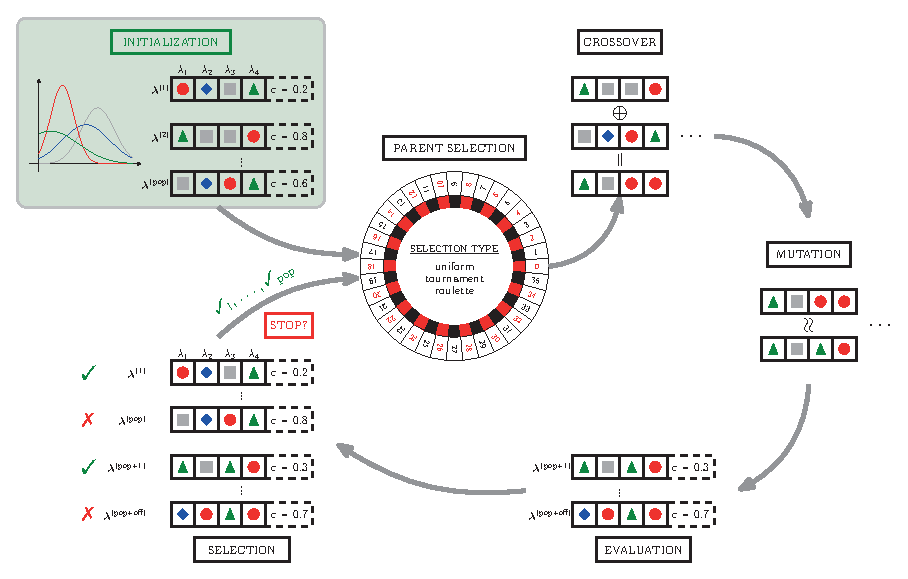
\includegraphics{figure_man/ea.eps}
\end{figure}

% \begin{figure}
% \centering
% \begin{tikzpicture}[node distance=1cm, auto,]
% %nodes
% \node (init) {Initialize population};
% \node[below = 0.3cm of init](rating1) {Eval population};
% \node[below = 0.3cm of rating1](selection1) {Parent selection};
% \node[below = 0.3cm of selection1](variation) {Variation};
% \node[below = 0.3cm of variation](rating2) {Eval offspring};
% \node[below = 0.3cm of rating2](selection2) {Survival selection};
% \node[below = 0.3cm of selection2](stop) {Stop};
% \node[below = 1cm of stop](dummy2) {};
% \node[below = 0.2cm of stop](dummy3) {};
% \node[right = 0.01cm of dummy3](dummy4) {yes};
% \node[left = 1.1cm of rating2](dummy1) {no};
% \draw[->] (init) to (rating1) node[midway, above]{};
% \draw[->] (rating1) to (selection1) node[midway, above]{};
% \draw[->] (selection1) to (variation) node[midway, above]{};
% \draw[->] (variation) to (rating2) node[midway, above]{};
% \draw[->] (rating2) to (selection2) node[midway, above]{};
% \draw[->] (selection2) to (stop) node[midway, above]{};
% \draw[->] (stop) to (dummy2) node[midway, above]{};
% \draw[->] (stop) to [bend left=90, looseness=2](selection1) node[midway, above]{};
% \end{tikzpicture}
% \end{figure}

\end{vbframe}

\begin{vbframe}{Notation and Terminology}

\footnotesize
\begin{itemize}
\item A chromosome is a set of parameters which encodes a proposed solution to the problem that the genetic algorithm is trying to solve. The chromosome is often represented as a binary string, although a wide variety of other data structures are also used.\\
\item The set of all solutions is known as the population.
\end{itemize}
\vspace{0.5cm}
\normalsize
\begin{center}
\begin{tabular}{ c | c}
    \textbf{Symbols} & \textbf{EA Terminology} \\[0.05cm]
    \hline \\[0.01cm]
    solution candidate $\bm{x}\in \mathcal{S}$ & Chromosome of an individual \\[0.1cm]
    $\bm{x}_j$  & $j$-th gene of chromosome\\[0.1cm]
    Set of candidates $P$ with $\mu = |P|$ & Population and size \\[0.1cm]
    $\lambda$ & Number of generated offsprings\\[0.1cm]
    $f: \mathcal{S} \to \R$ & Fitness function
\end{tabular}
\end{center}

\textbf{Note}: Unintuitively, we are minimizing fitness because we always minimize $f$ by convention.

% We now look into \textbf{operators}: Functions operating on (a set of) individuals and modifying 

%$$f(\bm{x}) = \widehat{GE}_{\mathcal{D}_{test}}\left(\inducer(\mathcal{D}_{train},\bm{x})\right)$$


\end{vbframe}

\begin{vbframe}{Encoding}

Encoding of chromosomes is the first step of solving a problem with EAs.  Technically: Mapping from \textbf{genotype} to \textbf{phenotype}. Encoding depends on the problem, and eventually decides performance of problem solving. 

\lz 

\textbf{Encoding methods}: 
\begin{itemize}
  \item Binary encoding: Strings of 0s and 1s 
  \item Real value encoding: Real values 

  \begin{figure}
    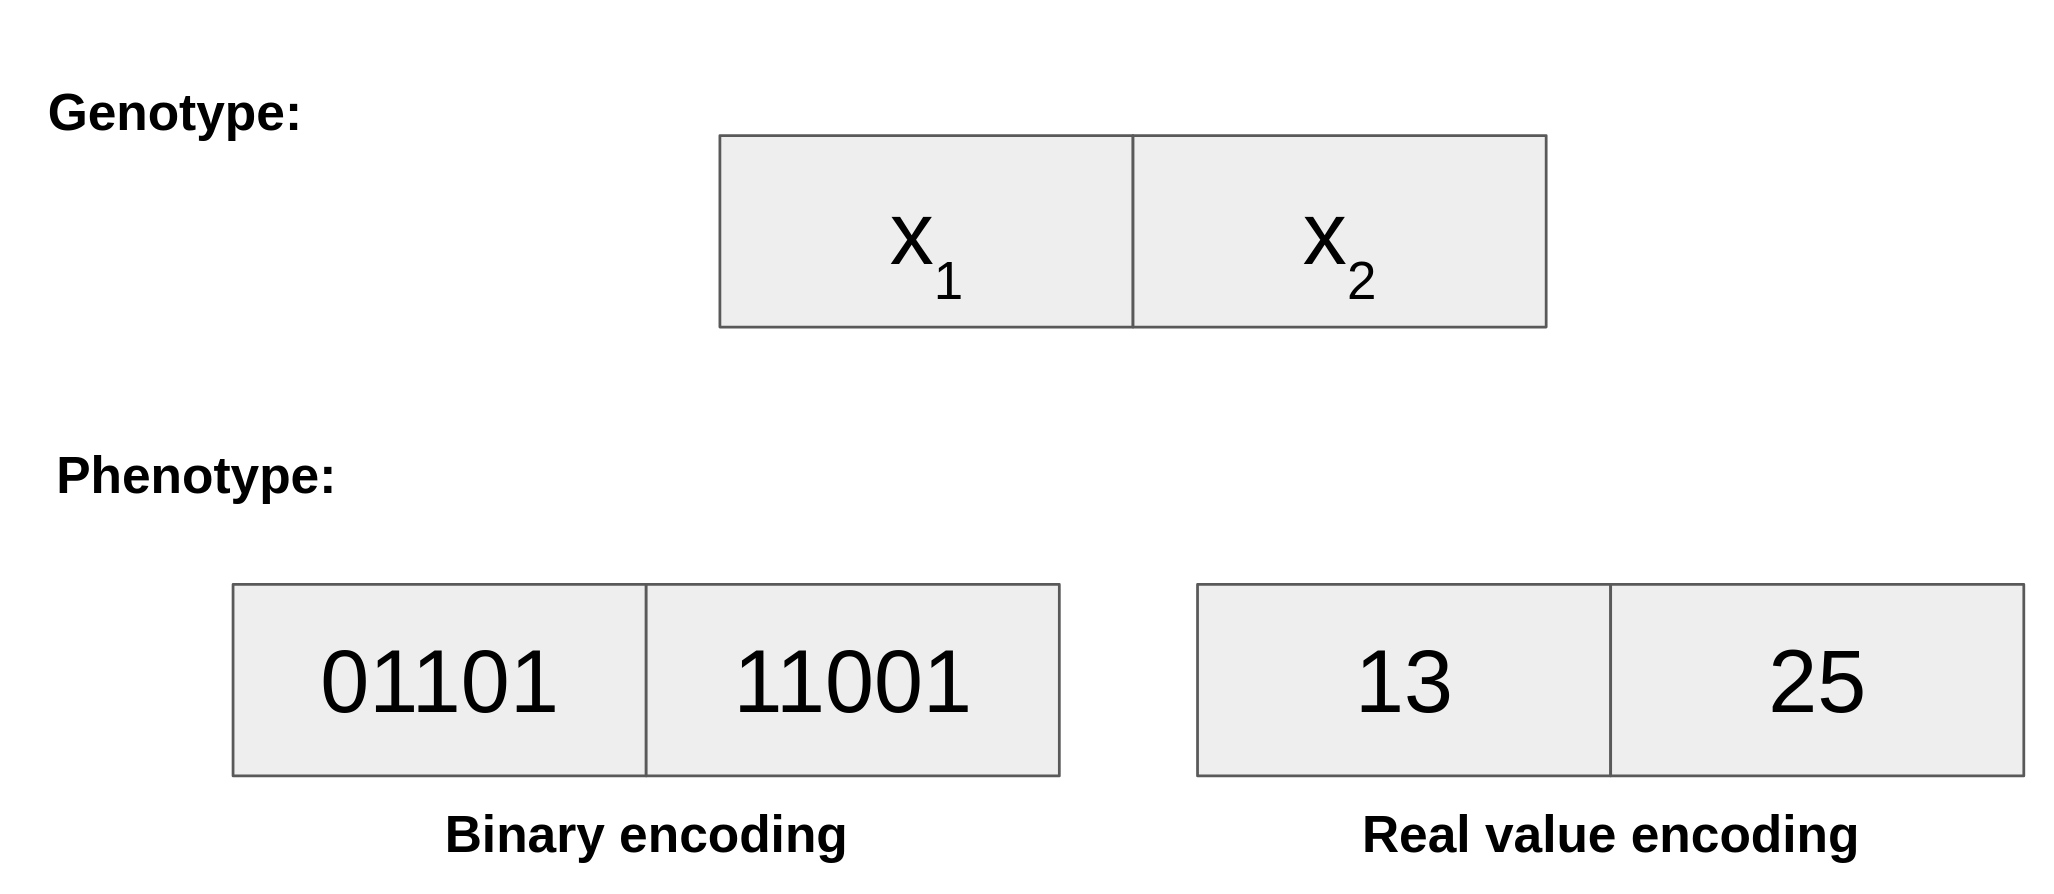
\includegraphics[width=0.7\textwidth]{figure_man/encoding_binary_numeric.png}
    % https://docs.google.com/presentation/d/12v81ZaLxJUgXVUBy3VdW0y6q7OKHS_6lFcQym3yeYsg/edit#slide=id.p
  \end{figure}
   %\item Order encoding: Sequence of elements 
  \item Tree encoding: Tree objects 
  \begin{figure}
    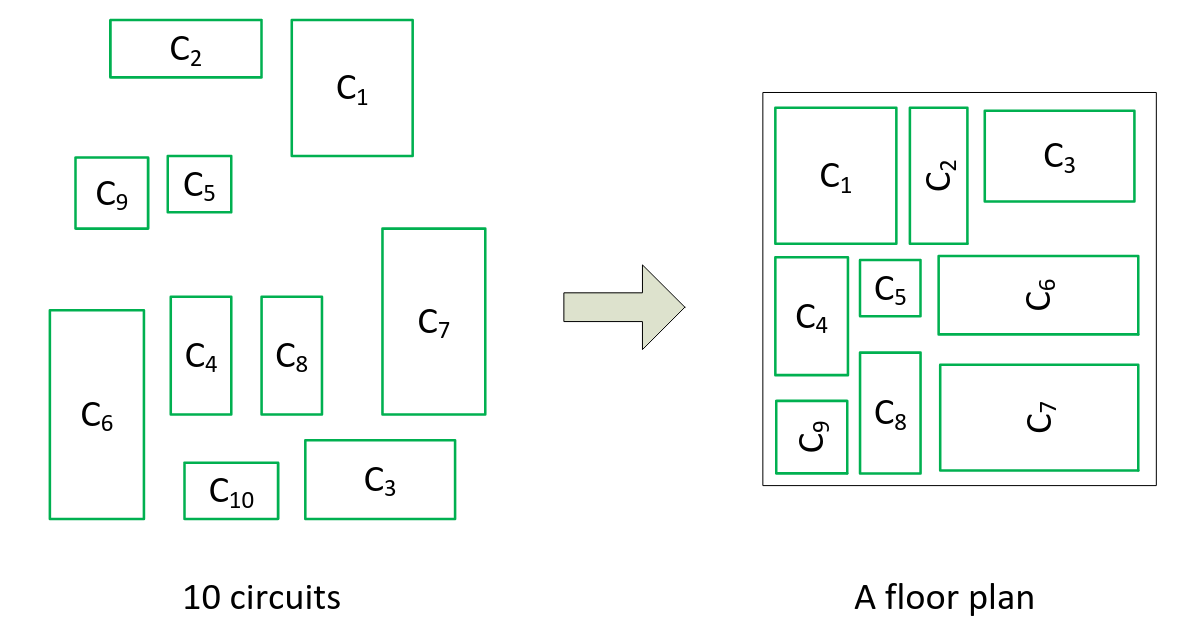
\includegraphics[width=0.45\textwidth]{figure_man/encoding_tree_1.png} ~~ 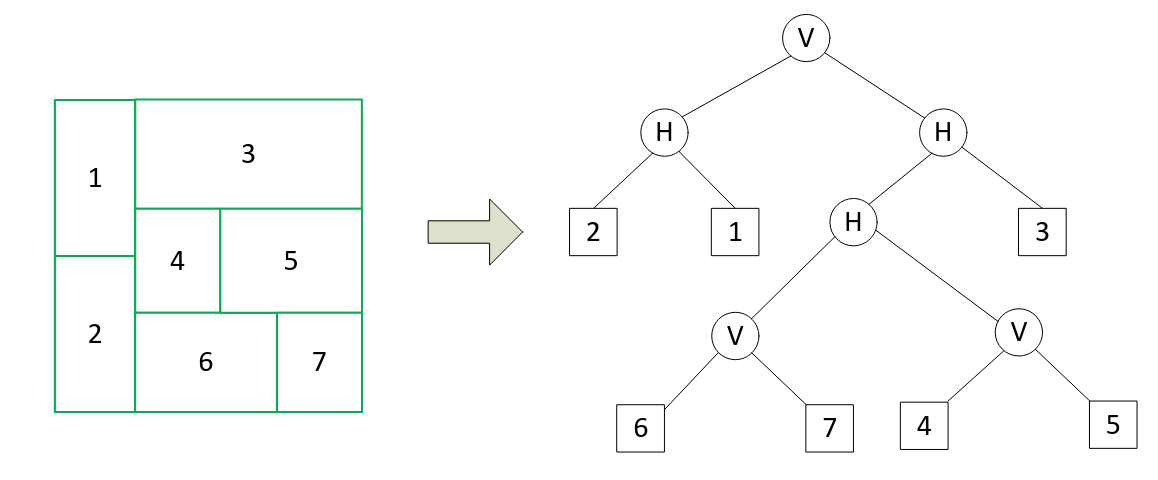
\includegraphics[width=0.45\textwidth]{figure_man/encoding_tree_2.png} \\
    \begin{footnotesize}
      Floor planning problem. Given are $n$ circuites of different area requirements. Goal: arrange them into a floor layour so that all curcuits are placed in a minimum layout possible. Each solution candidate can be represented by a tree. \\ 
      Souce: Encoding Techniques in Genetic Algorithms, Debasis Samanta, 2018. \\
      % https://cse.iitkgp.ac.in/~dsamanta/courses/sca/resources/slides/GA-02%20Encoding%20Techniques.pdf
    \end{footnotesize}
  \end{figure}
\end{itemize}

\end{vbframe}

\begin{vbframe}{Step 1: Initialize population}
    \begin{itemize}
            \item An evolutionary algorithm is started by generating an initial population $P = \{\bm{x}^{(1)}, ..., \bm{x}^{(\mu)}\}$.
            \item Usually, we sample this uniformly at random.
            \item We could introduce problem prior knowledge via a smarter init procedure.
            \item This population is evaluated, i.e., the objective function is computed for every individual in the initial population.
            \item The initialization can have a large influence on the quality of the found solution, so many EAs employ \textit{restarts} with new randomly generated populations.
    \end{itemize}

\end{vbframe}

\begin{vbframe}{Step 2: parent selection}
\footnotesize
The first step of an iteration chooses $\lambda$ parents, that create offspring for the next step.

\begin{itemize}
\item \textbf{Neutral selection: }choose individual with a probability $1/\mu$.
\item \textbf{Fitness-proportional / Roulette wheel selection: }draw individuals with probability proportional to their fitness.
\item \textbf{Tournament selection: }randomly select $k$ individuals for a "tournament group". Of the drawn individuals, the best one (according to fitness value) is then chosen. In order to draw $\lambda$ individuals, the procedure must be performed $\lambda$-times.
\end{itemize}
\vspace*{-0.2cm}
\begin{figure}
  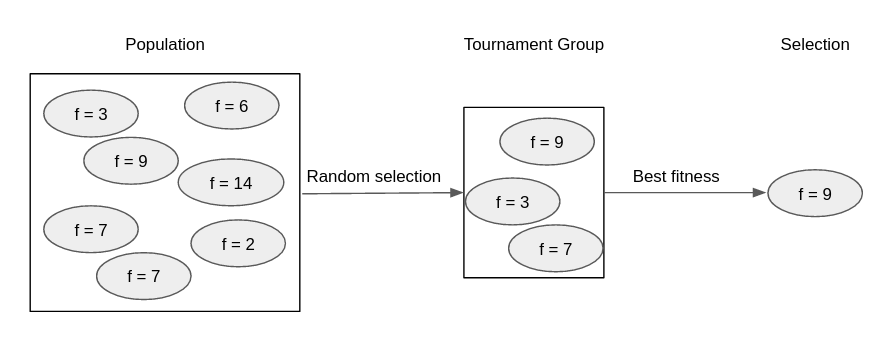
\includegraphics[width=0.5\textwidth]{figure_man/tournament_selection.png} 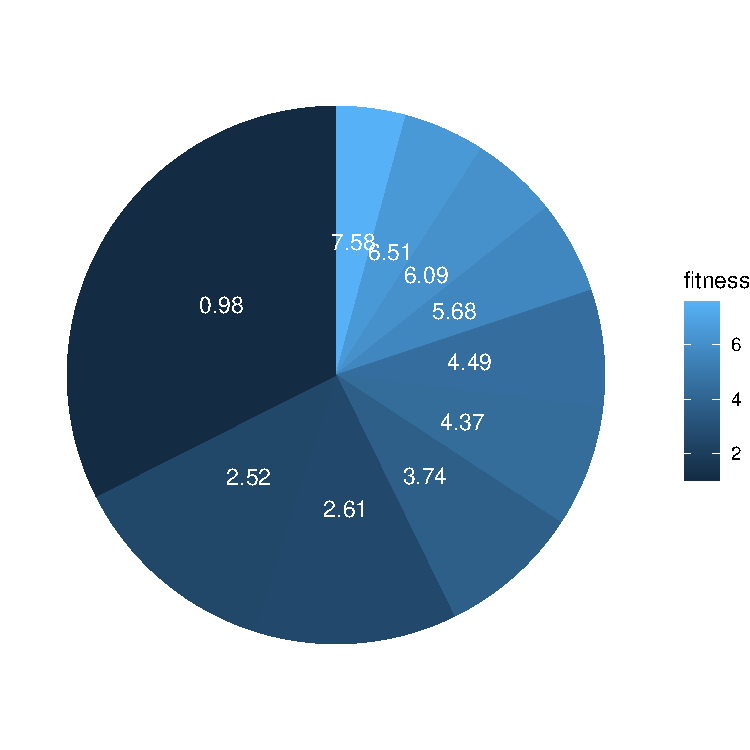
\includegraphics[width=0.3\textwidth]{figure_man/ea_parent_selection.pdf} \\
  \begin{footnotesize}
  Left: Random selection. Right: Fitness-proportional selection. Fitness values of $\mu = 10$ individuals (labels in pie-chart) are transferred inversely into probabilities (proportions of the pie-chart). 
  \end{footnotesize}
\end{figure}
\end{vbframe}

\begin{vbframe}{Step 3: variation}

New individuals are now generated from the parent population. This is done by

\begin{itemize}
\item Recombination/Crossover: combine two parents into one offspring.
\item Mutation: (locally) change an individual.
\end{itemize}

Recombination and mutation are not always performed both; sometimes only one operation is performed.

\vspace{0.3cm}
\begin{center}
\begin{figure}
  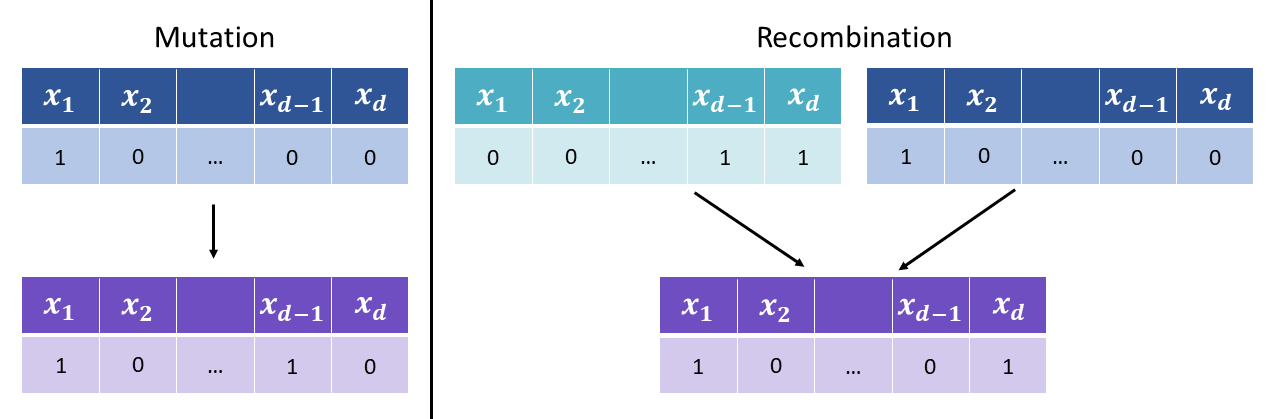
\includegraphics[width = 8cm, height = 2.6cm ]{figure_man/rec-and-mut.png}\\
\end{figure}
\end{center}

\textbf{Note: } The operation depends on the encoding. We will later look into examples for binary and numeric encodings. 

\end{vbframe}




  
\begin{vbframe}{Step 4: Survival selection}
  Now individuals are chosen who survive. Two common strategies are:
  \begin{itemize}
  \item \textbf{$(\mu, \lambda)$-selection:} We select from the $\lambda$ descendants the $\mu$ best ($\lambda \ge \mu$ necessary).\\
  \textbf{But:} best overall individual can get lost!
  \item \textbf{$(\mu + \lambda)$-selection:} $\mu$ parents and $\lambda$ offspring are lumped together and the $\mu$ best individuals are chosen.\\
  Best individual safely survives.
  \end{itemize}

\end{vbframe}



\begin{vbframe}{Evolutionary Algorithms}
\footnotesize
\textbf{Advantages}
  \begin{itemize}
    \item Conceptually simple, yet powerful enough to solve complex problems (including HPO)
    \item All parameter types possible in general
    \item Highly parallelizable (depends on $\lambda$)
    \item Allows customization via specific variation operators
  \end{itemize}
\textbf{Disadvantages}
    \begin{itemize}
      \item Less theory available (for realistic, complex EAs)
      \item Can be hard to get balance between exploration and exploitation right
      \item Can have quite a few control parameters, hard to set them correctly\\
      \item Customization necessary for complex problems
      \item Not perfectly suited for expensive problems like HPO, 
            as quite a higher number of evaluations is usually
            needed for appropriate convergence / progress
    \end{itemize}
    % \item Stagnation: Optimization process does not progress any more %FIXME: JR: Isn't that the same as the point below?
    % \item Premature Convergence: Algorithm converges to a single solution, which is not as good as expected
    % \item Diversity of population structures: Loss of population diversity for solving complex optimization problems

\end{vbframe}

%\begin{vbframe}{Example}

%In the following, methods for the individual steps of an evolutionary algorithm are presented.

%\lz

%These are demonstrated using the one-dimensional Ackley function, which we want to optimize on the $[-30, 30]$ interval.

%\lz

%In this case, each individual has exactly one chromosome. The chromosome is (obviously) encoded as a real number: $x_i \in \R$.

%\lz

%Usually for the optimization of a function $f:\R^n \to \R$ individuals are coded as real vectors $\bm{x}_i \in \R^n$.


%We start with a randomly selected population $\mathcal{P} = \{\bm{x}_1, ..., \bm{x}_\mu\}$ of the size $\mu = 20$ and rate it. The fitness function in this case is the function we want to minimize.

%\end{vbframe}


%\begin{vbframe}{Step 2: parent selection}
%\footnotesize
%In the first step of an iteration, $\lambda$ parents are chosen, who create offspring in the next step.

%\medskip

%Possibilities for selection of parents:
%\begin{itemize}
%\item \textbf{Neutral selection: }choose individual with a probability $1/\mu$.
%\item \textbf{Fitness-proportional selection: }draw individuals with probability proportional to their fitness.
%\item \textbf{Tournament Selection: }randomly select $k$ individuals for a "Tournament Group". Of the drawn individuals, the best one (with the highest fitness value) is then chosen. In order to draw $\lambda$ individuals, the procedure must be performed $\lambda$-times.
%\end{itemize}
%\vspace*{-0.2cm}
%\begin{figure}
%  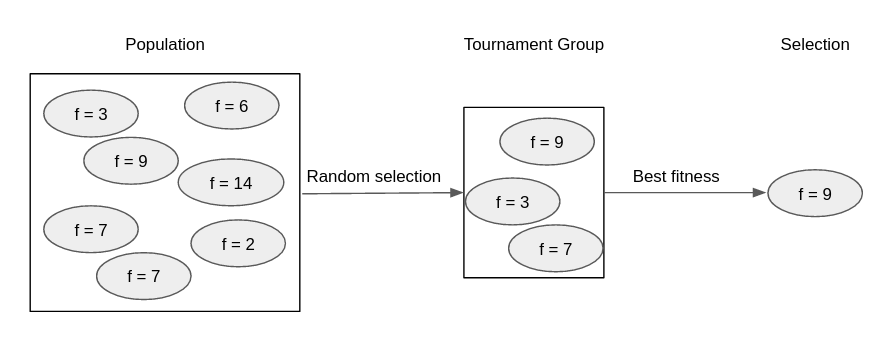
\includegraphics[width = 7cm, height = 2.5cm ]{figure_man/tournament_selection.png}
%\end{figure}
%\framebreak


%\begin{vbframe}{Mutation for numeric representations}

%\textbf{Mutation:} individuals are changed, for example for $\bm{x} \in \R^n$
%\begin{itemize}
%\item \textbf{Uniform mutation:} choose a random gene $x_i$ and replace it with a value uniformly distributed (within the feasible range).
%\item \textbf{Gauss mutation}: $\bm{\tilde x} = \bm{x} \pm \sigma \mathcal{N}(\bm{0}, \id)$
%\item \textbf{Polynomial mutation:} polynomial distribution instead of normal distribution

%\begin{center}
%\begin{figure}
 % 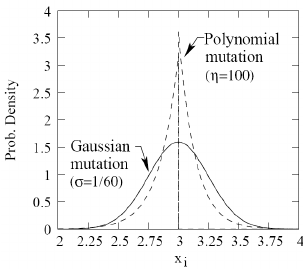
\includegraphics[height = 3.5cm, width = 4cm]{figure_man/polynomial_mutation.png}\\
  %\scriptsize{Source: K. Deb, Analysing mutation schemes for real-parameter genetic algorithms, 2014}
%\end{figure}
 %\end{center}

 %\framebreak

%More exact:

%$$
%{\tilde x_{i}} = x_{i} + (x_{i,upper} - x_{i,lower}) \delta_{i}
%$$

%with $x_{i,upper} (x_{i,lower})$ as upper (lower) bound for $x_{i}$.

%$\delta_{i}$ results as:

%\footnotesize
%$$
%\delta_{i} =
%\begin{cases}
%[2r_{i}+(1-2r_{i})(1-\delta)^{\eta_{m}+1}]^{\frac{1}{\eta +1}} -1, & r_{i} < 0.5 \\
%1 - [2(1-r_{i})+2(r_{i}-\frac{1}{2})(1-\delta)^{\eta_{m}+1}]^{\frac{1}{\eta_{m} +1}}, &  \text{else.}
%\end{cases}
%$$
%with  $\delta = \frac{min\{(x_{i} - x_{i,lower}), (x_{i,upper}-x_{i})\}}{x_{i,upper} - x_{i,lower}}$.

%\normalsize

%\lz

%Here $r_{i} \in [0,1]$ is a uniformly distributed number, $\eta_{m}$ is the distribution index of the mutation and is chosen by the user.\\
% Remark: A $\eta_{m}$ of the order of $\eta_{m} \in [20,100]$ is common.
%\normalsize
%\end{itemize}



%\lz

%In our example, we have chosen a Gauss mutation with $\sigma = 2$, we do not apply a recombination.


%\end{vbframe}

%\begin{vbframe}{Mutation for bit strings}

%For example, an individual $\bm{x} \in \{0, 1\}^n$ encoded as a bit string can be mutated as follows:

%\lz

%\textbf{Mutation:}
%\begin{itemize}
%\item \textbf{Bitflip}: for each index $k \in \{1, ..., n\}$: bit $k$ is flipped with probability $p \in (0,1)$.
%\item If $(a)$ is an arbitrary bit sequence to which a bitflip mutation is applied, $(b)$ is obtained.
%\end{itemize}

%\footnotesize
%\begin{center}
%\begin{tabular}{c @{\hspace{2\tabcolsep}} *{5}{c}}
 % &
%  \itshape (a) &
 % \itshape " " &
  %\itshape " " &
  %\itshape " " &
  %\itshape (b)

%\\[1ex]
%" " & 1 & " " & " " & "  " & \textcolor{red}{0}  \\
%" " & 0 & " " & " " & "  " & 0  \\
%" " & 0 & " " & $\Rightarrow$ & "  " & \textcolor{red}{1}  \\
%" " & 1 & " " & " " & "  " & \textcolor{red}{0}  \\
%" " & 1 & " " & " " & "  " & 1
%\end{tabular}
%\end{center}
%\normalsize

%\end{vbframe}



\endlecture
\end{document}

